%!TEX root = p.tex
\section{Query Engine}
Our query engine allows for arbitrary boolean query expressions to select a set of documents.  Documents can be matched based on metadata such as date, publication, or section title. They also can be matched based on whether the document contains a word form or named entity.  Each terminal item matches a subset of the entire corpus and returns a packed hit count for how many times that term matches the document.  Each internal item aggregates or filters its arguments.  Terms can also transform the type of the result sets from a list of document hit to a list of words or entities contained in those documents.  An example query in parsed form can be seen in figure \ref{fig:entity-query}.

\begin{figure}[htb]
  \centerline{
    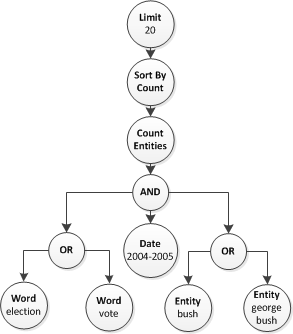
\includegraphics[width=40mm]{figures/entity-query.png}
  }
  \caption{A example query that returns the top 20 entities referenced in articles that mention the election of George Bush.}
  \label{fig:entity-query}
\end{figure}

Queries that return quantitative results, such as document hit counts, request a complete data matrix in a single request.  This minimizes overhead due to network latency and the limited number of simultaneous connections provided by a web-browser.  As shown in figure \ref{fig:json-query}, the queries have three main parameters: a global filter expression, an array of expressions to aggregate separately, and an array of buckets that filter documents into horizontal axis segments.

\begin{figure}[htb]
  \centerline{
    
\includegraphics[width=40mm]{figures/json-query.png}
  }
  \caption{An example query expression in 'JSON' using some syntactic sugar functions.}
  \label{fig:json-query}
\end{figure}

The query engine is built in Java using the Jersey RESTful web service framework.  Combining this framework with the Jackson JSON Processor allows for the automatic mapping of HTTP requests with a JSON payload into Java method calls that take Java objects as arguments.  This makes it very easy to build structured query expressions in Javascript and have them processed by the query service.

The query process runs in several phases, figures \ref{fig:query}, \ref{fig:pull}.  First all the input expressions are scanned and validated.  Once the query expression is validated, the series expressions that were submitted are crossed with the requested aggregation buckets to produce a family of query expressions.  Each one is submitted to the evaluator, which checks to see if it has recently processed any similar sub-expressions. If possible it reuses old results as it aggregates the results recursively.  Once the evaluator finishes, the specific logic for the query type applies any additional data transformations required by the front end, e.g. loading the article metadata for matching documents.

\begin{figure}[htb]
  \centerline{
    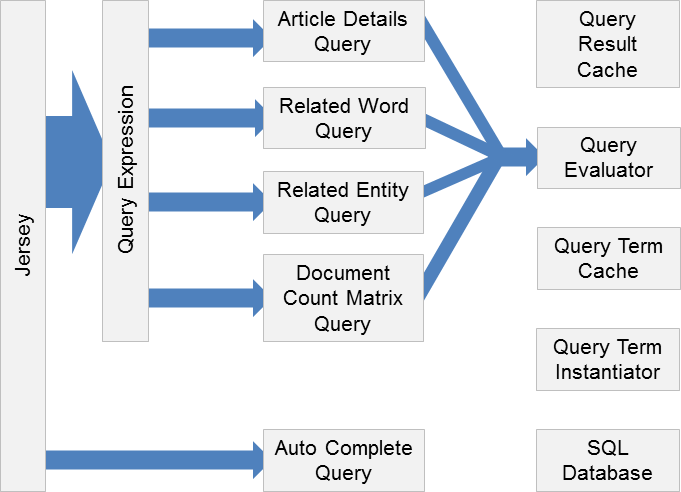
\includegraphics[width=60mm]{figures/query.png}
  }
  \caption{The four main query types are handled by the same query evaluator.}
  \label{fig:query}
\end{figure}

\begin{figure}[htb]
  \centerline{
    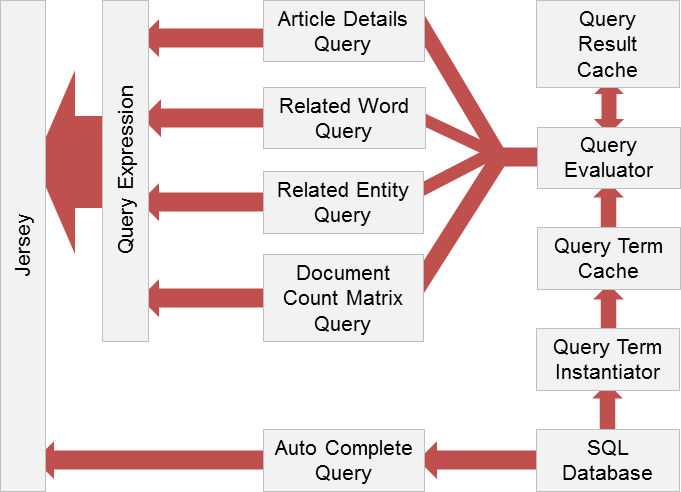
\includegraphics[width=60mm]{figures/pull.png}
  }
  \caption{The query evaluator pulls information from the SQL databasse into in memory caches and temporarily caches intermediate results to maximize interactivity.}
  \label{fig:pull}
\end{figure}


Terminal nodes imply a specific collection of documents, so the engine caches that intermediate state in memory using Java soft references.  If a term has not yet been seen, code is executed against the SQL database to generate the needed intermediate state.  Caching the sets of matching documents expressed by individual query terms allows for more interactive performance as queries are modified by the front end.  Typically, a query term will be reused many times as a user investigates a topic.

Some of the terms requires a large amount of data access to compute.  For example, computing the list of top entities over all documents in the corpus requires the entity list from all 2.5 million documents to be aggregated.  All of the database queries that load the entity list are tweaked to maximize the bandwidth that it can read from data.  Assuming there is adequate memory to allow for the database files to be cached in memory, the engine pulls over 2GB/s of data as it computes the results.  This entire query including data load and aggregation takes less than 15 seconds the first time it is executed, but that is still not fast enough for interactive performance.  The engine avoids needing to repeatedly perform similar hard queries by caching the results of each sub-expression that is evaluated.